\documentclass[../thesis/thesis.tex]{subfiles}
\begin{document}
 \chapter{Results}

 \section{Classifier Experiment Set 1}

\begin{table}
\centering
\begin{tabular}{|l|r|r|r|}
\hline
\textbf{Classifier}  & \textbf{\% Correct} & \textbf{RMS Error} & \textbf{F-Measure} \\ \hline
\multicolumn{4}{|c|}{\textit{Nominal Balanced}} \\ \hline
\textit{J48}         & 82.9                        & 0.2878             & 0.824              \\ \hline
\textit{KStar}       & 82.6                        & 0.2853             & 0.818              \\ \hline
\textit{Multilayer Perceptron}         & 78.5                        & 0.2936             & 0.777              \\ \hline
\textit{Naive Bayes} & 66.2                        & 0.3516             & 0.644              \\ \hline
\textit{IBk}         & 57.6                        & 0.4245             & 0.563              \\ \hline
\textit{SMO}         & 57.5                        & 0.3795             & 0.554              \\ \hline
\multicolumn{4}{|c|}{\textit{Nominal Unbalanced}} \\ \hline
\textit{J48}         & 78.5                        & 0.2771             & 0.784              \\ \hline
\textit{KStar}       & 74.4                        & 0.2926             & 0.743              \\ \hline
\textit{MLP}         & 71.9                        & 0.3285             & 0.718              \\ \hline
\textit{IBk}         & 68.8                        & 0.3715             & 0.670              \\ \hline
\textit{Naive Bayes} & 61.1                        & 0.3576             & 0.605              \\ \hline
\textit{SMO}         & 58.0                        & 0.3853             & 0.569              \\ \hline
\multicolumn{4}{|c|}{\textit{Numeric}} \\ \hline
\textit{Linear Regression}     & 63.4                        & 0.6589  &  -             \\ \hline
\textit{IBk}                   & 55.8                        & 1.1947  &  -          \\ \hline
\textit{Multilayer Perceptron} & 50.2                        & 0.7768  &  -          \\ \hline
\end{tabular}
\caption{Classifier Experiment Set 1 Results}
\label{tab:results:set1}
\end{table}

Experimental results from the first set of experiments were overall excellent, results from them can be seen in \Fref{tab:results:set1}. In the unbalanced results, an accuracy of 82.9\% was observed, and in the balanced results, 78.5\%. In the top balanced classifier, J48, the Root Mean Squared Error (RMSE) was 0.28 persons, a result better than Thermosense's 0.35 persons.

\begin{figure}
\centering
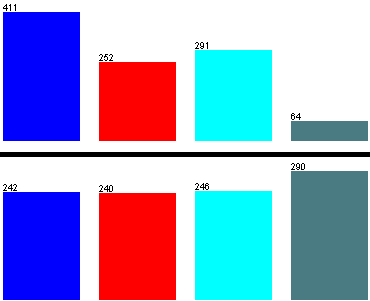
\includegraphics{../diagrams/temp/resample.png}
\caption{Experiment Set 1 Class Distribution Before and After Re-sampling}
\label{fig:results:resample}
\end{figure}

Between the unbalanced and balanced classes, the ranking of different algorithms remained approximately the same, and consistently dropped in accuracy, with the exceptions being SMO, which increased in accuracy by 0.5\% in that instance, and, more notably, IBk, which increased in accuracy by 11.2\%. The drop in accuracy can be explained mostly by an over-representation of the zero class within the under-balanced data, and an underrepresentation of the three class (see \Fref{fig:results:resample}). These biases would enable classes to over-predict and under-predict these two classes respectively and achieve an artificially higher accuracy as a result. As discussed in the Methods, we performed re-sampling inside Weka to compensate for this.

For the numeric representation of the number of people, accuracy was consistently poor. In this instance, we calculate the ``correctly classified'' percentage by taking the predicted vs. actual results from Weka and rounding the predicted values to whole numbers, as a theoretical real-world solution may do to finalize its prediction. From this data, we can see that all three classifiers used performed consistently poorly, with the Root Mean Square Errors being consistently double or more of comparable nominal results. Interestingly, IBk was on-par with its nominal unbalanced partner, while the Multi-Layer Perceptron's accuracy dropped by more than 30\%.

For the Linear Regression model, the most striking difference to the Thermosense paper is evident. While Thermosense claims an RMSE of 0.409, our results show a much poorer 0.659, a difference of more than 46\%. Looking more closely at the Linear Regression generated, \Fref{eq:linreg}, we can see that the impact of the three features on the model are minimal, with the algorithm choosing minuscule weights. This suggests that the algorithm was unable to find any strong correlation between the three features and the number of people. 

\begin{equation} \label{eq:linreg}
n = 0.0783a + -0.0616b + -0.0331c + 0.4923
\end{equation}

%The two highest accuracy classifiers, J48 and KStar, share very similar 

 \ifcsdef{mainfile}{}{\bibliography{../references/primary}}
\end{document}
